%%%%%%%%%%%%%%%%%%%%%%%%%%%%%%%%%%%%%%%%%%%%%%%%%%%%%%%%%%%%%%%%%%%
%
% This is the LaTeX source for the paper we plan to submit to
% HPEC'17. It is formatted for publication with the IEEE.
%
% Page limit for HPEC is 6 pages not counting references.
%
%%%%%%%%%%%%%%%%%%%%%%%%%%%%%%%%%%%%%%%%%%%%%%%%%%%%%%%%%%%%%%%%%%%

\documentclass[conference]{IEEEtran}
\usepackage{amssymb}
\setcounter{tocdepth}{3}
\usepackage[caption=false]{subfig}
\usepackage{graphicx}
\usepackage{subfig}
\usepackage{listings}
\usepackage{enumitem}
%\usepackage{hyperref}
\newcommand{\url}[1]{#1}
\usepackage{todonotes}

\usepackage[colorlinks=true, 
	bookmarks=true,        %%% generate bookmarks ...
	bookmarksnumbered=true,%%% ... with numbers
	hypertexnames=false,%              %%% needed for correct links to figures !!!
	breaklinks=true,%                  %%% breaks lines, but links are very small
	pdfborder={0 0 0 0}]{hyperref}%  %%% border-width of frames
	
\graphicspath{{../figures/}}
\DeclareGraphicsExtensions{.pdf,.jpeg,.png,.jpg,.eps}

% correct bad hyphenation here
\hyphenation{op-tical net-works semi-conduc-tor}

\newcommand{\eg}{\emph{e.g.}}
\newcommand{\ie}{\emph{i.e.}}

\begin{document}

\pagestyle{plain}

\title{GraphBLAS C API: \\ Ideas for future versions of the specification}

%
% Name order to reflect whoever puts the most work into the paper
%
\author{\IEEEauthorblockN{
         Timothy G. Mattson\IEEEauthorrefmark{1},
         Carl Yang\IEEEauthorrefmark{2},
         Scott McMillan\IEEEauthorrefmark{3},        
         Ayd{\i}n Bulu\c{c}\IEEEauthorrefmark{4},
         Jos\'e E. Moreira\IEEEauthorrefmark{5}
       }
%
% affiliations ... order matters
       \vspace{1ex}
\IEEEauthorblockA{
	\IEEEauthorrefmark{1}Intel Corporation, Hillsboro OR, USA ({\tt timothy.g.mattson@intel.com}) \\
     \IEEEauthorrefmark{2}University of California, Davis CA, USA ({\tt ctcyang@ucdavis.edu}) \\
     \IEEEauthorrefmark{3}Software Engineering Institute, CMU, Pittsburgh PA, USA ({\tt smcmillan@sei.cmu.edu}) \\
     \IEEEauthorrefmark{4}Lawrence Berkeley National Laboratory, Berkeley CA, USA ({\tt abuluc@lbl.gov}) \\
     \IEEEauthorrefmark{5}IBM Corporation, Yorktown Heights NY, USA ({\tt jmoreira@us.ibm.com})}
}
%%%%%
\maketitle
\thispagestyle{plain}
%%%%%
\begin{abstract}
The GraphBLAS C specification provisional release 1.0 is complete. To
manage the scope of the project, we had to defer important functionality
to a future version of the specification.  For example, we are well
aware that many algorithms benefit from an inspector-executor execution
strategy.  We also know that users would benefit from a number of standard
predefined semirings as well as more general user-defined types. These
and other features are described in this paper in the context of a future
release of the GraphBLAS C API.
\end{abstract}
%%%%%
%%%%%%%%%%%%%%%%%%%%%%% file intro.tex %%%%%%%%%%%%%%%%%%%%%%%%%
%
% This file contains the introduction section of the paper
%
%%%%%%%%%%%%%%%%%%%%%%%%%%%%%%%%%%%%%%%%%%%%%%%%%%%%%%%%%%%%%%%%%%%
\section{Introduction}
\label{sec:intro}
The GraphBLAS are great and you'll love them.  In this paper, we'll talk about the even greater stuff coming in the future
%%%%%
%%%%%%%%%%%%%%%%%%%%%%% file GrBDescrip.tex %%%%%%%%%%%%%%%%%%%%%%%%%
%
% This file contains the description of GraphBLAS C API
%
%%%%%%%%%%%%%%%%%%%%%%%%%%%%%%%%%%%%%%%%%%%%%%%%%%%%%%%%%%%%%%%%%%%

\renewcommand{\vector}[1]{{\bf #1}}
\renewcommand{\matrix}[1]{{\bf #1}}

%%%%%
\section{The GraphBLAS C API}
\label{sec:GrBCspec}

This section gives a brief overview of important elements 
of Version 1.0 of the GraphBLAS C API specification in order give some context 
for future extensions proposed in this paper.  More details of the API can be 
found in \cite{graphblas_capi_17}, or the full specification can be downloaded 
from the GraphBLAS Forum website \cite{graphblas_web}.  Like the original BLAS, 
this library performs operations on matrices and vectors.  However there are 
significant differences to specifically support graph operations as described 
in \cite{mathgraphblas16}. 

\begin{figure}[b]
\hrule
\footnotesize
\[
\matrix{C}\langle \matrix{M} \rangle ~ [\odot] = ~ \matrix{A}^{[T]} \oplus.\otimes \matrix{B}^{[T]}
\]
\begin{center}(a) The mathematical definition.\end{center}

\begin{verbatim}
GrB_Info GrB_mxm(GrB_Matrix               C,
                 const GrB_Matrix         M,  
                 const GrB_BinaryOp       accum,
                 const GrB_Semiring       op,
                 const GrB_Matrix         A, 
                 const GrB_Matrix         B,
                 const GrB_Descriptor     desc);
\end{verbatim}
\begin{center}(b) The function signature.\end{center}
\caption{GraphBLAS matrix-matrix multiply operation: {\sf mxm}.\label{Fig:mxmfig}}
\hrule
\end{figure}

Since nearly all operations in the API follow the same basic structure, we will
highlight important aspects of the API by examining one operation: matrix-matrix
multiply as shown in Figure~\ref{Fig:mxmfig}.  Figure~\ref{Fig:mxmfig}(a) illustrates
the mathematical notation for that operation (optional items in brackets). This is similar to what is found in
\cite{mathgraphblas16}, with some additions supported by the API -- write masks and
accumulation -- which are contained in the signature in Figure~\ref{Fig:mxmfig}(b).
In the signature for every GraphBLAS operation, the output argument always 
appears first. This is followed by the write mask and accumulate operation, if supported. 
Next, the arguments describing the input objects and the math to be performed are
listed. Finally, the last argument is the optional descriptor.  All GraphBLAS methods
return a status code ({\sf GrB\_Info}) regarding the success of the call.

\subsection{Objects}

At its foundation, the GraphBLAS C API is built on opaque data types exposed
through the API by handles.  
A few of these opaque types are collections -- matrices and vectors --
where matrices are typically very sparse and vectors can be
sparse as well.  The {\sf mxm} signature consists of one output matrix, {\sf C}, and 
two input matrices, {\sf A} and {\sf B}. The dimensions and 
domain (type) of the object are specified at construction time and remain fixed for the lifetime of 
the object.  A number of domains corresponding to the C built-in types are
supported, and the API allows for definition of user-defined types as well.

The GraphBLAS C API also has opaque types for algebraic objects including
unary and binary operators, monoids, and semirings, which differ from the traditional
linear algebra of the BLAS.  The traditional arithmetic addition and
multiplication operations can be replaced (e.g., min and plus, respectively) through
user-defined capabilities that can operate on data from multiple domains.  The {\sf op} 
argument in Figure~\ref{Fig:mxmfig} corresponds to a GraphBLAS semiring, denoted by $\oplus.\otimes$ in the 
mathematical description, and it specifies the binary operations that take the 
place of arithmetic addition and multiplication, respectively. The {\sf accum}
argument in the signature, denoted by $\odot$, is an optional binary operator that can
be used to combine the results with existing values in the output matrix. If accumulation
is not desired, {\sf GrB\_NULL} is specified.

The API supports a few optional control objects: write masks and descriptors.  A
mask is specified using GraphBLAS matrix (or a vector for 1-dimensional operations).
Since this is a write mask, it is applied when assigning results to the output matrix
{\em after} accumulation has been performed.
The descriptor is a lightweight object that can modify the semantics of the
operation by allowing the user to specify which input parameters need to be transposed
prior to the operation, whether the mask should be structurally complemented, or whether
the output should be cleared before assignment.
Note that {\sf GrB\_NULL} can be specified if default behavior is desired.

\subsection{Operations}

The API supports the basic operations that were outlined in \cite{mathgraphblas16}:
inserting and extracting data, matrix multiply, element wise operations, subgraph assignment
and extraction, apply, reduction, and transpose.  It also provides a number of
variants that are useful in a number of graph algorithms. For example, instead of
just row reduction of a matrix to a vector, the API also supports reduction of both
matrices and vectors to scalars.  Another example is the ability to assign a constant
scalar value to an entire subgraph (through a variant of subgraph assignment). 

\subsection{Execution Models}

The API also supports two executions modes: blocking and nonblocking. In blocking mode,
each API method completes the operation before proceeding to the next.  However, 
because the API is meant to support high-performance computing in a parallel and
distributed environment we also provide a non-blocking mode.  In this mode, the methods
{\em may} return immediately after the input arguments have been verified but before
any computation has been carried out.  This mode gives an implementation the flexibility
to choose an execution strategy that might reduce computation time through fused
operations, lazy evaluation, asynchronous evaluation, and/or asynchronous execution.  When
using nonblocking mode, a slightly different mechanism is used for reporting errors which
is beyond the scope of this paper.

%%%%%
\section{Standard Definitions}
\label{Sec:stddef}

\newcommand{\integer}{{\sf int32\_t}}
\newcommand{\float}{{\sf float}}
\newcommand{\double}{{\sf double}}
\newcommand{\bool}{{\sf bool}}
\newcommand{\false}{{\sf false}}
\newcommand{\true}{{\sf true}}

The current GraphBLAS specification could be augmented with a list of 
pre-defined objects, such as descriptors, semirings and monoids, that are commonly used
in building graph algorithms. These standard pre-defined objects would
simplify coding and ensure more consistency across algorithms. 
We emphasize
that individual application writers are always free to create their own set of
pre-defined objects.

Additionally, GraphBLAS could include pre-defined macros that support
shorter calling syntax for methods, by hiding default arguments. 
Again, individual application writers are always free to create their
own set of pre-defined macros.

We propose that such pre-defined objects and macros would
be included in a compilation unit by including a header file as follows:

\begin{verbatim}
  #include <GrB_stddef.h>
\end{verbatim}

Table~\ref{Tab:stddef} shows an initial set of proposed standard object
definitions.  It includes descriptors for transposing either or both input
matrices, Boolean monoids and the standard arithmetic monoids for integer,
single-precision floating-point and double-precision floating-point
data.  It also includes the conventional Boolean semiring, as well as
arithmetic semirings for integer, single-precision floating-point and
double-precision floating-point data.  Other semirings commonly used
with graph algorithms can also be added.

\begin{table}[bt]
	\hrule
	\caption{Initial set of proposed standard definitions for GraphBLAS.}
	\label{Tab:stddef}
	\begin{center}
	\begin{tabular}{|l|l|} \hline
		 Name				& Description \\ \hline
         Descriptors: & \\
				{\sf GrB\_TA}			& ${\sf GrB\_INP0} = {\sf GrB\_TRAN}$ \\
                {\sf GrB\_TB}			& ${\sf GrB\_INP1} = {\sf GrB\_TRAN}$ \\ 
				{\sf GrB\_TATB}		& ${\sf GrB\_INP0} = {\sf GrB\_INP1} = {\sf GrB\_TRAN}$ \\
				{\sf GrB\_TASR}		& ${\sf GrB\_INP0} = {\sf GrB\_TRAN}$, \\
							& ${\sf GrB\_MASK} = {\sf GrB\_SCMP}$, \\
							& ${\sf GrB\_OUTP} = {\sf GrB\_REPLACE}$ \\ \hline
		Monoids:	& \\
				{\sf GrB\_Lor}		& $\left\langle \bool, \vee, \false \right\rangle$ \\
				{\sf GrB\_Land}		& $\left\langle \bool, \wedge, \true \right\rangle$ \\
				{\sf GrB\_FP32Min}		& $\left\langle \float, {\sf min}, \infty \right\rangle$ \\
				{\sf GrB\_FP32Max}		& $\left\langle \float, {\sf max}, -\infty \right\rangle$ \\
				{\sf GrB\_Int32Add}		& $\left\langle \integer, +, 0 \right\rangle$ \\
                {\sf GrB\_Int32Mul}		& $\left\langle \integer, \times, 1 \right\rangle$ \\
				{\sf GrB\_FP32Add}		& $\left\langle \float, +, 0.0 \right\rangle$ \\
				{\sf GrB\_FP32Mul}		& $\left\langle \float, \times, 1.0 \right\rangle$ \\
				{\sf GrB\_FP64Add}		& $\left\langle \double, +, 0.0 \right\rangle$ \\ 
				{\sf GrB\_FP64Mul}		& $\left\langle \double, \times, 1.0 \right\rangle$ \\ \hline
		Semirings:	& \\
				{\sf GrB\_Boolean}		& $\left\langle \bool, \bool, \bool, \vee, \wedge, \false \right\rangle$ \\
                {\sf GrB\_Int32AddMul}	& $\left\langle \integer, \integer, \integer, +, \times, 0 \right\rangle$ \\
				{\sf GrB\_FP32AddMul}		& $\left\langle \float, \float, \float, +, \times, 0.0 \right\rangle$ \\ 
				{\sf GrB\_FP64AddMul}		& $\left\langle \double, \double, \double, +, \times, 0.0 \right\rangle$ \\ 
                {\sf GrB\_FP32MinPlus}	& $\left\langle \float, \float, \float, {\sf min}, +, \infty \right\rangle$ \\\hline
	\end{tabular}
	\end{center}
	\hrule
\end{table}

\label{sec:stddefs}
%%%%%
\section{Inspector-Executor}

In its non-blocking mode of execution, GraphBLAS allows specific
implementations to support various alternative execution approaches. In
particular, it allows for methods to be executed in
several stages, possibly interleaved with stages from other methods. This
is called \emph{split execution}. In a particular split execution, a
method can go through an \emph{analyze} stage followed by a \emph{perform}
stage.  The analyze stage computes various characteristics of the object
being produced, whereas the perform stage does the actual calculations.

It may be desirable to augment GraphBLAS with additional constructs to
control this particular analyze/perform split explicitly. In particular,
having the application communicate properties of an object that do not
change between multiple perform stages greatly simplifies
or eliminates the need for analyze stages.

As a concrete example, the current GraphBLAS specification exposes {\sf
mxm} as a single operation to the user. Under the hood, it is understood
that {\sf mxm} is typically implemented in two phases: analyze and
compute. The analyze phase consists of allocating memory to the output
matrix. The compute phase computes the value at each nonzero of the
output matrix. The implementer has the option of deciding whether to
set the nonzero structure of the output matrix in the analyze phase or
the compute phase.

It may be desirable in some circumstances to expose these two phases of
{\sf mxm} to the user explicitly. There are a few options on how to do that, 
including separate methods and leveraging the functionality of the descriptor. 
(See Section~\ref{Sec:Extensions}.)

For typical use cases, neither the size nor the nonzero structure of the output
matrix \textbf{C} are known \emph{a priori} before the {\sf mxm}
operation is run. However, there may exist situations where the user is
computing a sequence of output matrices \textbf{C} which share
the same nonzero structure and memory layout. In this case, it may be advantageous for the user to 
explicitly call both the analyze and compute phases 
for the first matrix-multiplication
in the sequence, and only the compute for the rest.

We used two experimental testbeds to test the importance of \emph{split
execution} for {\sf mxm} operation. Experiments were performed on a
quad-core Intel Xeon CPU E5-2637 v2 @ 3.50GHz with 256 GB RAM running
Ubuntu 14.04.1, and an NVIDIA K40c GPU with 12 GB RAM. Some more details
of the test setups are listed in Table~\ref{Tab:testbed}.

For our datasets (see Table~\ref{Tab:testset}), we chose
six matrices from the University of Florida Sparse Matrix
Collection~\cite{davis2011university} because they come from diverse
sources (epidemic modeling, finite element modeling, protein data,
web connectivity) and have varying sparsity structures ranging from
fairly regular (\emph{epidemiology}, \emph{wind tunnel}, \emph{protein},
\emph{sphere}) to highly irregular (\emph{hood}, \emph{webbase}). To
test the above mentioned use case, we compared calling {\sf mxm} ten
times with no split execution, to a split execution where a call to {\sf
mxm} analyze phase is followed by ten calls to {\sf mxm} compute phase.

Performance of the test cases is shown in Figure~\ref{Fig:gflops}. We observe that the split
execution performs better than the unsplit execution. MKL sees a geometric mean
37.2\% speedup going to split execution, while cuSPARSE sees a geometric mean
29.3\% speedup. In general, cuSPARSE performed better than MKL on the
larger datasets (\emph{wind tunnel}, \emph{protein} and \emph{sphere}),
but worse on the smaller ones (\emph{epidemiology} and \emph{webbase}).

\begin{table}[htb]
	\hrule
	\caption{Experimental setup used for benchmarking.}
	\label{Tab:testbed}
	\begin{center}
		\begin{tabular}{|c|c|c|} \hline
			Vendor & Intel & Nvidia \\ \hline
			Family & Xeon & Tesla GPU \\
			Device & E5-2637 v2 & K40c \\
			Codename & Sandy Bridge & Kepler GK110 \\
			Memory & 256 GB & 12 GB \\
			OS & Ubuntu 14.04.1 & Ubuntu 14.04.1 \\
			Compiler & Intel C++ v17.0.4 & nvcc v8.0.44 \\
			& Intel OpenMP v5.0 & g++ v4.9.4 \\
			Library & Intel MKL 2017.4.196 & cuSPARSE v8.0.44 \\ 
			API & mkl\_Scsrmultcsr & cusparseScsrgemm2 \\ \hline
		\end{tabular}
	\end{center}
	\hrule
\end{table}

\begin{table}[htb]
	\hrule
	\caption{Description of datasets used for benchmarking. Flops refers to the number of floating-point computations required to square the matrix by itself. Two copies of the matrix are kept in memory for sake of benchmarking.}
	\label{Tab:testset}
	\begin{center}
		\begin{tabular}{|c|c|c|c|c|} \hline
			Dataset & Rows & Nonzeros & Flops & Symmetric\\ \hline
			\emph{epidemiology} & 526k & 2.1M & 16.8M & no \\
			\emph{wind tunnel} & 218k & 11.6M & 1.3B & yes \\
			\emph{protein} & 36k & 4.3M & 1.1B & yes\\
			\emph{sphere} & 83k & 6.0M & 0.9B & yes\\
			\emph{hood} & 221k & 10.8M & 1.1B & yes \\
			\emph{webbase} & 1.0M & 3.1M & 139M & no \\ \hline
		\end{tabular}
	\end{center}
	\hrule
\end{table}

\begin{figure}
	\centering
	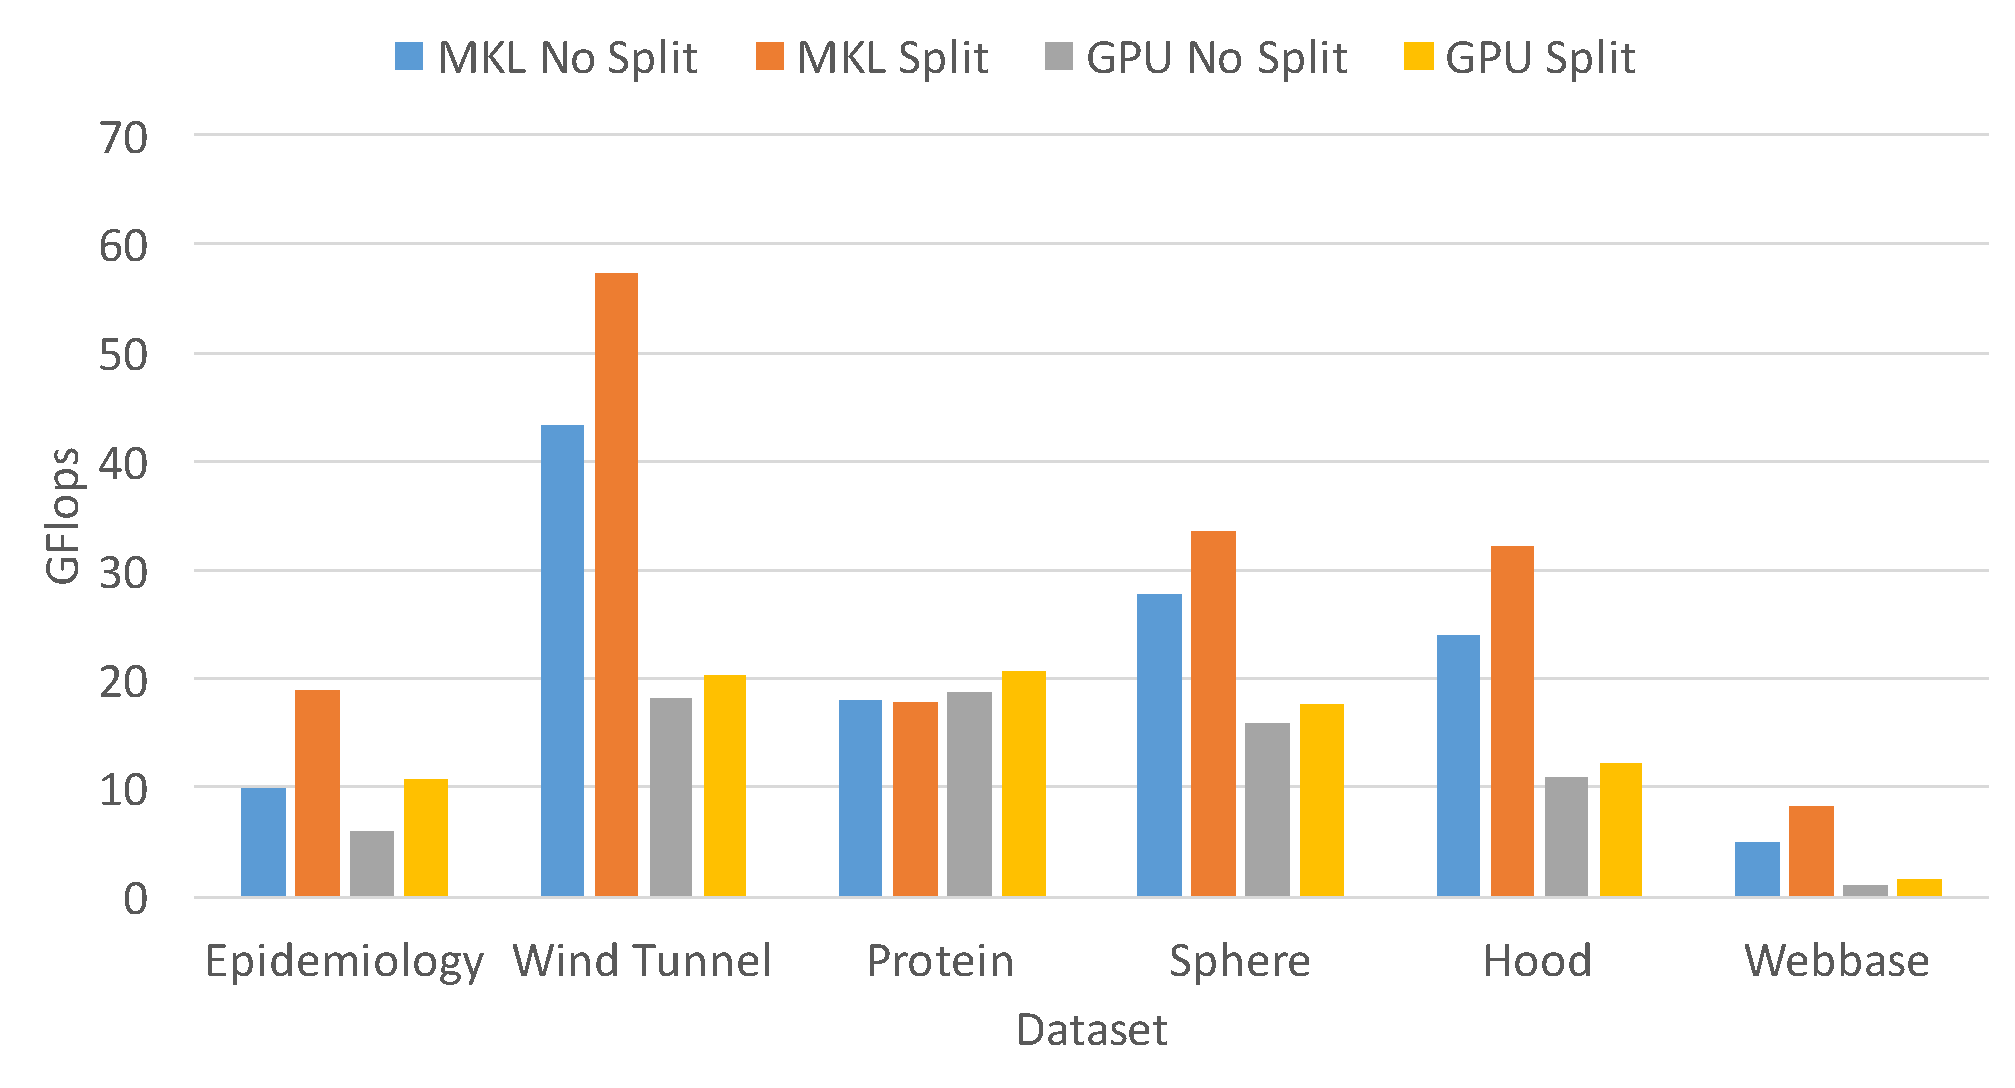
\includegraphics[width=.9\linewidth]{gflops.pdf}
	\caption{Comparison of {\sf mxm} runtime with and without split execution for two experimental setups, MKL and cuSPARSE.}
	\label{Fig:gflops}
\end{figure}

We decided to defer such facilities from version 1.0 of the GraphBLAS specification. There is a computational benefit to the user in being able to access split execution, but the API will need to become more complex in order to support it. We believe that additional experience with implementation and use of GraphBLAS is necessary before we can define the proper interfaces for explicit split execution.

\label{sec:inspecExec}
%%%%%
\section{Dependency DAGs and {\sf wait} on Specific Objects}
\label{Sec:DAG}

In the current specification of GraphBLAS, when operating in \emph{nonblocking
mode}, the operation {\sf wait} will ensure that the current sequence of
GraphBLAS operations has either completed successfully, or encountered an
error. Further, a sequence in nonblocking mode where every GraphBLAS
operation is followed by an {\sf wait} call is equivalent to the same
sequence in blocking mode with {\sf wait} calls removed.

It may be desirable to modify the {\sf wait} interface such that it
takes a GraphBLAS object as parameter, and performs all
outstanding computations needed to compute that particular object.
This approach gives the programmer finer grained specification of the synchronization,
while giving the GraphBLAS implementation more flexibility in scheduling operations.

We decided to defer such an interface from version 1.0 of the GraphBLAS
specification. We believe that additional experience with implementing and
using GraphBLAS nonblocking mode is necessary before we
can determine what is the best approach.

\label{sec:dag}
%%%%%
%%%%%%%%%%%%%%%%%%%%%%%%%%%%%%%%%%%%%%%%%%%%%%%%%%%%%%%%%%%%%%%%%%%
\section{API-transparent Extensions}
\label{Sec:Extensions}

A defining characteristic of the GraphBLAS C API is its use of
\emph{descriptors} to modify the behavior of a method.  In the current
definition of the API descriptors can specify preprocessing steps for
input data (typically, whether an input matrix should be transposed or
not before the operation) as well as controlling how the result value
is written to the output object (complement or not the mask, preserve
or not the elements that are masked).

This descriptor-based approach allows one to extend the functionality of
methods without changing their interface, since all main GraphBLAS methods
already include an optional descriptor as the last argument. We envision
some new uses for descriptors in future versions of the GraphBLAS C API.

First, we plan to provide a {\sf GrB\_STRUCTURE\_ONLY} modifier for masks.
In the present specification of GraphBLAS, masks need to be matrices
or vectors of a predefined type. And only those elements of a mask
that evaluate to a boolean {\sf true} value are considered active.
Specifying {\sf GrB\_STRUCTURE\_ONLY} in the {\sf GrB\_MASK} field of
a descriptor would direct GraphBLAS to consider all elements present
in the mask as active, irrespective of their value.  As a side effect,
vectors and matrices of any type could be used as masks.

Another item under consideration is the use of assertions about the
properties of the output object. Those assertions could be used to
implement optimizations for certain operations. For example, specifying
{\sf GrB\_FIXED\_STRUCTURE} in the {\sf GrB\_OUTP} field of a descriptor
would assert that the output object will not change structure (pattern
of nonzero elements) during this operation. Therefore, computation
can happen in place with new values simply replacing old values. This
would accomplish similar optimization results as achieved by a split
analyze/compute execution. Moreover, a spectrum of standard properties,
from more restrictive to more permissive can be specified. For example,
{\sf GrB\_SYMMETRIC} can assert that the output is a symmetric matrix,
whereas {\sf GrB\_FIXED\_NVALS} can assert that the number of elements
in the output is constant (even though the structure may change).

In the case of assertions, it is important to specify how \emph{hard}
or \emph{soft} those assertions are. That is, do they cause a run-time
error if violated or are they just ``hints'' that the implementation
can use to improve performance but should be able to recover from,
maybe with big performance penalties, if they prove to be wrong.

\label{sec:masks}
%%%%%
\section{Generalized User-Defined Types}
\label{Sec:UsrTypes}

Currently, GraphBLAS only supports a limited form of user-defined
types. In particular, objects of the data type must have a flat memory
representation, so that two objects can be copied with a simple {\tt
memcpy} operation.  It is desirable to lift this restriction. One
possibility would be to add a version of {\sf GrB\_Type\_new} that
supports arbitrary user-defined types as follows.

When the user creates a new type, he or she must pass three functions
that perform the most basic operations in that type:
\begin{enumerate}
	\item A \emph{create} function that creates an object of the
	user-defined type. That includes allocating storage for the
	object and initializing that object to a default state.

	\item A \emph{copy} function that copies the state of a source
	object of the user-defined type to a target object of the same
	user-defined type.

	\item A \emph{destroy} function that destroys an object of the
	user-defined type, releasing any resources the object uses.
\end{enumerate}
Optionally, we could allow create, copy and destroy methods for arrays
of user-defined objects, in order to avoid the overhead of function
calls and memory management at the level of each individual object.
The description of this new form of {\sf GrB\_Type\_new} is shown
in Figure~\ref{Fig:GrB_Type_new}.

\begin{figure}
\hrule
\footnotesize
\paragraph{Syntax}

\begin{verbatim}
GrB_Info GrB_Type_new(GrB_Type   *utype,
                      void       *create,
                      void       *destroy,
                      void       *copy);
\end{verbatim}

\paragraph{Parameters}

\begin{itemize}[leftmargin=0.6in]
\item[{\sf utype}] ({\sf INOUT}) On successful return, contains a handle to the newly created user-defined GraphBLAS type object.
\item[{\sf create}] ({\sf IN})    A pointer to a function that creates and initializes (to a default state) an object of the user-defined type. Such function must return a {\tt void*} pointer to the new object. Its signature is \verb|void* create()|.
\item[{\sf destroy}] ({\sf IN}) A pointer to a function that destroys an object of the user-defined type, releasing any resources the object uses. Its signature is \verb|void destroy(void* obj)|.
\item[{\sf copy}] ({\sf IN}) A pointer to a function that copies the contents from a source object of the user-defined type to a destination object of the same user-defined type. Its signature is \verb|void copy(void* tgt, const void* src)|.
\end{itemize}

\paragraph{Return Values}

\begin{itemize}[leftmargin=1.6in]
\item[{\sf GrB\_SUCCESS}]           operation completed successfully.
\item[{\sf GrB\_PANIC}]             unknown internal error.
\item[{\sf GrB\_OUT\_OF\_MEMORY}]          not enough memory available for operation.
\item[{\sf GrB\_NULL\_POINTER}]    at least one of {\sf utype}, {\sf create}, {\sf destroy}, {\sf copy} pointers is {\sf NULL}.
\end{itemize}

	\caption{Definition of a {\sf GrB\_Type\_new} GraphBLAS method that can support arbitrary user-defined types.}
	\label{Fig:GrB_Type_new}
\hrule
\end{figure}

\label{sec:usrTypes}
%%%%%
 \section{Kronecker Product}
\label{Chp:Extensions}
One of the proposed operations in the mathematical specification of GraphBLAS is Kronecker product. It is not present in the current GraphBLAS API, but may be added in the future. Kronecker product may be useful for generating graphs. It is known that the Kronecker product of the adjacency matrices of two graphs is the adjacency matrix of their tensor product graph.


\label{sec:kronProd}
%%%%%
\section{Rank Promotion}
\label{Sec:promotion}

\renewcommand{\vector}[1]{{\bf #1}}
\renewcommand{\matrix}[1]{{\bf #1}}

\emph{Rank promotion} is the conversion of an object of lower rank (\eg,
scalar or rank 0) to an object of a higher rank (\eg, vector or rank 1).
It is a common feature in array programming languages suchs as Fortran~90+
and MATLAB.  Typically, a scalar is converted to a matrix or vector
by replicating it in every element of the matrix or vector. A vector is
conveterd to a matrix by replicating it either along the rows or along the
columns of the matrix.  The replication factor can be stated explicitly
or implicitly calculated in order to result in a valid operation.

In GraphBLAS, scalars, whether of built-in or user-defined type, are
always of rank 0. Vectors and matrices are of rank 1 and 2, respectively.
Our proposal is to support \emph{automatic} rank promotion by allowing,
in most cases, the use of an object of lower rank in an input argument.

For example, in the GraphBLAS matrix multiply method 
\begin{quote} 
{\sf GrB\_mxm(C,Mask,accum,op,A,B,desc)}
\end{quote}
{\sf A} and {\sf B} are input matrices. One could replace either (or both)
of them by a scalar or vector.  Assume no tranposition specified by the
descriptor {\sf desc}, and let {\sf C} be an $m \times n$ matrix, {\sf A}
be a scalar and {\sf B} be an $p \times n$ matrix. The scalar {\sf A}
would be converted into an $m \times p$ matrix, with all its elements
set to the value of {\sf A}.  After that, the matrix multiplication would
proceed as specified in the standard.  We note that the same requirements
for domain compatibility would still hold.

If, instead, {\sf A} were an $m$-element vector, it would be converted into
an $m \times p$ matrix by replicating it $p$ times as a column of the matrix.
Replication as rows could be achieved by specifying transposition of
{\sf A} in the descriptor.

A tentative list of GraphBLAS methods supporting automatic rank
promotion is shown in Table~\ref{Tab:Promotion}. We should note that 
rank promotion can already be accomplished explicitly with the existing
GraphBLAS methods. However, doing it automatically, as we propose,
saves a matrix or vector instantiation just for that purpose.

\begin{table}[htb]
	\hrule
	\caption{Tentative list of automatic rank promotions in GraphBLAS.}
	\label{Tab:promotions}
	Matrices: $\matrix{A},\matrix{B},\matrix{C},\matrix{M}$ \\
	Vectors: $\vector{a},\vector{b},\vector{u},\vector{w}$ \\
	Scalars: $a,b,u$ \\
	$\Delta$ denotes a descriptor \\
	$\mathbb{S}$ is a semiring \\
	$\odot$ is a binary operator used for accumulation \\
	\begin{center}
		\begin{tabular}{|l|l|} \hline
			Method		& Promotions \\ \hline
			${\sf GrB\_mxm}(\matrix{C},\matrix{M},\odot,\mathbb{S},\matrix{A},\matrix{B},\Delta)$	& $a \rightarrow \matrix{A}$ \\
														& $\vector{a} \rightarrow \matrix{A}$ \\
														& $b \rightarrow \matrix{B}$ \\
														& $\vector{b} \rightarrow \matrix{B}$ \\
			\hline
			${\sf GrB\_vxm}(\vector{w},\matrix{m},\odot,\mathbb{S},\vector{u},\matrix{A},\Delta)$	& $u \rightarrow \vector{u}$ \\
														& $a \rightarrow \matrix{A}$ \\
                                                                                                                & $\vector{a} \rightarrow \matrix{A}$ \\
			\hline
			${\sf GrB\_mxv}(\vector{w},\matrix{m},\odot,\mathbb{S},\matrix{A},\vector{u},\Delta)$	& $u \rightarrow \vector{u}$ \\
														& $a \rightarrow \matrix{A}$ \\
                                                                                                                & $\vector{a} \rightarrow \matrix{A}$ \\
			\hline
		\end{tabular}
	\end{center}
	\hrule
\end{table}

\label{sec:promotion}
%%%%%
\section{Conclusion}
\label{sec:conclusion}

The C binding to the GraphBLAS standard is excellent and will have a huge 
impact on the development of Graph Algorithms.


%%%%%
\newpage
%%%%%%%%%%%%%%%%%%%%%%% file results.tex %%%%%%%%%%%%%%%%%%%%%%%%%
%
% This file contains the acknowledgments and the Intel federal mandated disclaimer
%
%%%%%%%%%%%%%%%%%%%%%%%%%%%%%%%%%%%%%%%%%%%%%%%%%%%%%%%%%%%%%%%%%%%

\section*{Acknowledgments and Disclaimers}

We thank the members of the GraphBLAS forum.

This material is based upon work funded and supported by the Department of 
Defense under Contract No. FA8702-15-D-0002 with Carnegie Mellon University for 
the operation of the Software Engineering Institute, a federally funded research 
and development center [DM17-0410].


%%%%%
\bibliographystyle{abbrv}
\bibliography{GrB}
%%%%%
\end{document}
